\listfiles
\documentclass[a4paper,11pt]{report}

\author{Vladislav K. Valtchev} 
\title{IHPP: An Intraprocedural Hot Path Profiler}


\usepackage[utf8]{inputenc}
\usepackage[english]{babel}

\usepackage{hyperref}
\usepackage{xcolor,graphicx}
\usepackage{mdwlist}
\usepackage{fix-cm}
\usepackage{array}
\usepackage{tikz}
\usepackage{wrapfig}
\usepackage{listings}
\usepackage{cite}
%\usepackage[lighttt]{lmodern}
\usepackage{bold-extra}
\usepackage{cleveref}
%%%%%%%%%%%%%%%%%%%%%%%%%%%%%%%%%%%%%%%%%%%%%%%%%%%%%%%%%%%%%%%

\usetikzlibrary{arrows,graphs,trees,fit,shapes,backgrounds}

\hypersetup{
    colorlinks,
    citecolor=black,
    filecolor=black,
    linkcolor=black,
    urlcolor=black
}

\lstset{
	basicstyle=\ttfamily\small, 
	basewidth=0.5em,
	tabsize=4,
	keywordstyle=\bfseries,
	captionpos=b,
	framesep=10pt,
	numbersep=15pt
}


%in order to make the analytical index
%\usepackage{makeidx}
%\makeindex

\pagestyle{headings}

\begin{document}

\thispagestyle{empty}

\begin{figure}
\centering

\includegraphics[scale=0.6]{logo}
\end{figure}


\begin{center}


{\Large\textsc{Universit\`a degli studi di Roma}\\} 
{\huge\textsc{La Sapienza}\\[10pt]}
{\huge\textsc{Facolt\`a di Ingegneria}\\[40pt]} 

{\large Tesi di laurea in: \\}
{\LARGE\textsc{Ingegneria Informatica}\\[30pt]}

{\LARGE \textbf{IHPP}\\[10pt]\textit{An \textbf{I}ntraprocedural \textbf{H}ot \textbf{P}ath \textbf{P}rofiler}}\\[50pt]


\begin{tabular*}{0.9\textwidth}{@{\extracolsep{\fill}} @{} c @{} c @{} }
{\normalsize Docente relatore: } & {\normalsize Autore:}\\
{\large \textit{Prof. Camil Demetrescu} } & {\large \textit{Vladislav K. Valtchev}}\\
\end{tabular*}

\mbox{}\\[90pt]

{\large Anno accademico: 2011/2012\\}


\end{center}

%in order to print the analytical index
%\printindex

\pagebreak

%\thispagestyle{empty}
%
%\begin{center}
%
%\vspace*{4.5cm}
%
%\fontsize{70}{90}\selectfont \textbf{IHPP}\\
%\fontsize{20}{35}\selectfont
%\textit{An \textbf{I}ntraprocedural \textbf{H}ot \textbf{P}ath \textbf{P}rofiler}\\
%
%\vspace{11cm}
%
%\fontsize{14}{20}\selectfont
%\textbf{Vladislav K. Valtchev}
%
%\end{center}
%\pagebreak

\begin{abstract}
dwehkhjrkweh rlkewrhwe lkrhwek rhwel krhjweklrh welkrh wekrhwe krhwr
werwerwekr h jwekj rhwk jrhwk rhwl kjrh k kqhe qe wrkjehr r hk rhj
wlhrwelkjrfh sd hf kjh sdfkh jq ql lkqjhekqj q eqhkjeqkj kjahq 
erhjwe skafhd lkaerh welrk liwer  iwerh wit wielr qierhu lqr 
dwehkhjrkweh rlkewrhwe lkrhwek rhwel krhjweklrh welkrh wekrhwe krhwr
werwerwekr h jwekj rhwk jrhwk rhwl kjrh k kqhe qe wrkjehr r hk rhj
wlhrwelkjrfh sd hf kjh sdfkh jq ql lkqjhekqj q eqhkjeqkj kjahq 
erhjwe skafhd lkaerh welrk liwer  iwerh wit wielr qierhu lqr 
dwehkhjrkweh rlkewrhwe lkrhwek rhwel krhjweklrh welkrh wekrhwe krhwr
werwerwekr h jwekj rhwk jrhwk rhwl kjrh k kqhe qe wrkjehr r hk rhj
wlhrwelkjrfh sd hf kjh sdfkh jq ql lkqjhekqj q eqhkjeqkj kjahq 
erhjwe skafhd lkaerh welrk liwer  iwerh wit wielr qierhu lqr 
dwehkhjrkweh rlkewrhwe lkrhwek rhwel krhjweklrh welkrh wekrhwe krhwr
werwerwekr h jwekj rhwk jrhwk rhwl kjrh k kqhe qe wrkjehr r hk rhj

\end{abstract}


\tableofcontents

\chapter{Introduction}

In a world like today's one where computers are everywhere and where
\mbox{Internet} has more than 2.2 billion users, software has become more
important than ever. Today's operating systems have to handle much more
processes than in the past and every single process is often much more ``heavy''
than before due a great deal of reasons including (but not limited to): the
demand of users for much more complicated tasks (for example the multimedia
related ones), the intensive use of software layers by the programmers, the use
of high-level interpreted languages and many others. Thus, even if performance
of hardware is still growing following Moore's law and actual computers are
thousands times faster than before, they still to be ``slow'' sometimes and
software still needs to be analyzed and optimized. One way of analyzing
performance of programs is \textbf{profiling}: it consists substantially in
running the target program in a controlled environment and collecting data about
its behavior in order to discover possible bottlenecks in software. A basilar
introduction of program analysis and various profiling techniques can be found
in chapter 2.

\section{Actual profilers}

There are many profiler types today and a discrete number of profilers for
each category (as readers can see in the next chapter). But, \emph{most of them}
have two characteristics in common:

\begin{itemize*}

\item They focus only on procedures: data such counters and timers are collected
only on the procedure basis. This means that there is no way to understand what
happened \emph{inside} the procedures which caused, for example, a bottleneck.

\item Data has almost no \emph{calling context}, for example: it is possible to know that
a function \verb|a()| was called 10 times in a certain program, but it is not possible to know which were the \emph{callers} of \verb|a()|. Some profilers like \textbf{Valgrind} can
produce data with 2 levels of context: this means it is possible to know, for
example, that \verb|a()| was called 10 times, 3 of them by function
\verb|b()| and 7 of them by function \verb|c()|. This is better, but sometimes
it is not enough.

\end{itemize*}

Even if it is not too difficult to collect data with full context (infinite
levels) which is called ``building a CCT'' \emph{(calling context
tree)}, this often is practically useless because it grows too much specially due to
functions recursion~\cite{kccf}: the CCT is often too big to be physically stored and copied
simply and it is too big to be human-analyzable.
Thus, in the last years a few researches in theoretical computer science 
proposed different approaches for solving this problem and collecting \textbf{not fully context-sensitive} data. IHPP, the project described in this paper, uses one of these approaches called \textbf{$k$-CCF} (after explained).

\section{Motivations}

The aim of creation of IHPP was to make something that allows the study of
function calls with an arbitrary number of calling contexts but also to go
beyond the concept of procedure-only profiling: IHPP uses same ideas of
procedure-profiling to study the execution flow of basic blocks \emph{inside}
 functions. This sometimes can be really useful when there is a bottleneck in
the algorithm used for solving a problem: the programmer already knows which are
the \emph{slow functions} but he is still unaware of \emph{where exactly}
the problem is. Imagine functions with 3 loop levels and many conditional
statements: it is not trivial to understand where the problem is, neither to
solve it. But, even if a profiler \emph{will not} tell the programmer \emph{how}
to solve the problem, it will tell \emph{quickly} where is it, which is much
better than nothing because it can save several hours of programmer's work.

\section{Contributions}

In order to collect k-level context-sensitive data, IHPP uses some data
structures and algorithms that \emph{have not been} ideated by the author:

\begin{itemize*}
\item k-SF \emph{(k-Slab Forest)}
\item k-SF construction algorithm\footnote{This algorithm is used in the \textbf{traceObject()} function}
\item k-CCF \emph{(k-Calling Context Forest)}
\item Forest join and inversion operations\footnote{These two operations should
be intended as \emph{theoretical} operations: in IHPP concrete algorithms have been
developed by the author}
\end{itemize*}

For these great and innovative data structures and algorithms, the author warmly
thanks \emph{Giorgio Ausiello}, \emph{Camil Demetrescu}, \emph{Irene Finocchi}
and \emph{Donatella Firmani}, professors at the \emph{Sapienza University of
Rome}\footnote{Officially, \textbf{Universit\`a degli studi di Roma ``La
Sapienza''}}. Their work, called \emph{\mbox{k-Calling Context Profiling}}, has
been accepted for the \emph{27th \mbox{ACM SIGPLAN} Conference on
Object-Oriented Programming, Systems, Languages and Applications (OOPSLA 2012)}.

\section{Thesis structure}

\chapter{Program analysis}
The short introduction of before used the concept of \emph{profiling} without
too many explanations.
Instead, the goal of this chapter is to explain a \emph{little more} about
profiling contextualizing it in the more general concept of program analysis.
This kind of \emph{scientific background} has an encyclopedic form and
absolutely has no claim to be a good and an exhaustive coverage about the
subject since it is not the purpose of this paper.

Program analysis is the process of analyzing the behavior of computer
programs. Main applications of program analysis are 
\emph{program correctness checking} and \emph{program optimization}.
There are two main approaches in program analysis: static analysis and dynamic analysis.
The main difference between them is that in \emph{static} analysis nothing is
executed: the analysis is conducted only by observing the program source code or
the compiled program instructions. Instead, the \emph{dynamic} program analysis
is based on executing the program and observing what is it doing, even in real
time if possible.

\section{Static analysis}

Static analysis can be done either by hand or by using another program.
Information obtained by static analysis can be used in many ways, from
highlighting possible coding errors to application of formal methods that
mathematically prove some required properties of the algorithms used. It is
necessary to say, even if this is not the right context, that, as the work of
Alan Turing proved, there is no way to prove the absolute
correctness of an arbitrary program because of the \emph{halting
problem}~\cite{Turing01}.
By the way, there are many methods that give us estimated solutions with a
good level of reliability. We can mention four ways of doing static program
analysis:


\begin{description}
\item[Model checking] considers systems that have finite state or may be reduced to finite state by abstraction
\item[Data-flow analysis] is a lattice-based technique for gathering information about the possible set of values
\item[Abstract interpretation] models the effect that every statement has on the
state of an abstract machine (i.e., it 'executes' the software based on the
mathematical properties of each statement and declaration)
\item[Use of assertions] in program code as first suggested by Hoare
logic~\cite{Hoare01}
\end{description}

A more in deep explanation of these approaches goes too far away from the purpose of this paper.

\section{Dynamic analysis}

Dynamic program analysis is a form of analysis substantially based on the execution of the \emph{target program} in a sort of ``controlled environment''.
This definition is a quite generic because there many different ways of doing
this type of analysis as there are different objectives that who does the
analysis wants to achieve. For example, it can be done in order to trace memory
allocations (and discover memory leaks), to discover race conditions, memory
corruption, security vulnerabilities and also to do a \emph{performance
analysis}, which is often called \textbf{profiling}. It is usual to refer as \emph{profiling} when
the final goal of the work is to improve the program  \emph{performance} and
not, for example, to improve program \emph{correctness}: a memory analysis
is always a dynamic analysis but is not always a form of \emph{profiling}.

\subsection{The profiling}
The profiling is probably the most common form of dynamic program analysis and
its goal is, to analyze the performance of a program: the
\emph{performance} can be the amount of memory used, the frequency of certain
instructions, the frequency and/or the time consumption of some
\emph{procedures} / \emph{basic blocks} inside certain procedures. 
It is interesting here to focus the attention on the last kind of profilers; 
they can classified in two ways: according to the type of output and according to the method of data acquisition. Using the first classification rule, the following distinctions can be done:

\begin{description}
\item[Flat profilers] \hfill \\
These profilers count the number of function calls and/or average cpu time used
by each function without keeping trace of the calling context of the function.
\item[Call-graph profilers] \hfill \\
These profilers do the same things flat profilers do but also produce in output
the call-chains involved on the callee, which means that it is possible to know,
at the end of the execution of the target program, for every function, say it
$f()$, which functions were called by $f()$, which functions were
callers of $f()$ and how many times each function called each other. With this
information, it is possible to draw a
\emph{call-graph} like the one in figure~\ref{callgraph1}. But, this is
\emph{not} calling context profiling (which is what \textbf{IHPP} does) because,
for example, there is information such: $f()$ called $b()$ 8 times and $f()$ was called 20
times, 5 by $x()$ and 15 by $y()$ but there is \emph{not info} about how many times the
distinct calling sequence $x()\rightarrow f()\rightarrow b()$ occurred and how
many times the other calling sequence $y()\rightarrow f()\rightarrow b()$
occurred.

\begin{figure}

\begin{center}

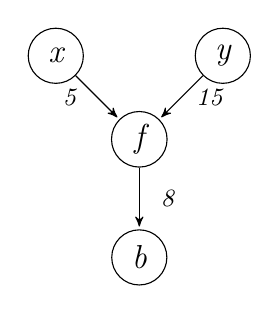
\begin{tikzpicture}
[->,>=stealth',shorten >=1pt,
node distance=1.5cm,
minimum size=7mm,
main node/.style={circle, draw, font=\itshape\large}]

  \node[main node] (1) {x};
  \node[main node] (3) [below right of = 1] {f};
  \node[main node] (2) [above right of = 3] {y};
  \node[main node] (4) [below of = 3] {b};

  \path[every node/.style={font=\itshape\small}]
    
    (1) edge node [left] {5} (3)
    (2) edge node [right] {15} (3)
    (3) edge node [right] {8} (4);
    
\end{tikzpicture}

\end{center}

\caption{A call graph}
\label{callgraph1}

\end{figure}



\end{description}

\begin{flushleft}
Instead, classifying profilers according to the method of data acquisition:
\end{flushleft}


\begin{description}
\item[Event-based profilers] \hfill \\
Some high-level languages and frameworks have they ad-hoc profilers based on
events. For example, \textbf{Java} has \textbf{JVMPI} \textit{(Java Virtual
Machine Profiling Interface)}, while in \textbf{.NET} it is possible to attach a
profiling agent as COM server to a .NET program using the \emph{Profiling APIs}.
These profilers are called \emph{event-based} because statements (of the
relative intermediate language) like function calls (or returns), object
creations (and many others \ldots) have \emph{traps} handled at low-level by the
relative virtual machine which generates \emph{events} and propagates these ones
to the high-level user event-handlers objects.

\item[Statistical profilers] \hfill \\
This kind of profilers work by \emph{sampling} at regular intervals the
\emph{instruction pointer} of target program through \emph{software interrupts}.
This approach, of course, produces numerically approximate data, but allows the
program to run at near full speed. Common profilers of that kind are \textbf{AMD
CodeAnalyst}, \textbf{Apple Shark}, \textbf{Intel VTune} and \textbf{Intel
Parallel Amplifier}.

\item[Instrumentation profilers] \hfill \\
This kind of profilers are used for \emph{native programs}\footnote{A native
program is a program written in a compiled language like \textbf{C},
\textbf{C++}, \textbf{Pascal}: the result of the building is an executable
containing architecture-specific instructions. Instead, non-native programs (aka
managed programs) don't contain binary instructions: they contain
intermediate-language (IL) instructions which only the relative virtual machine
(VM) understand. In order to the program to run, their VM runtime compile IL
instructions into machine specific instructions. \textbf{Java} and \textbf{.NET}
technologies use intermediate languages called relatively \textbf{Bytecode} and
\textbf{MSIL}.} and need to add binary instructions to the target program in
order to ``catch events'' like function calls. Instrumentation profilers can be
classified by the way they ``add instructions'' to the target program:

\begin{description}
\item[Manual]
This approach consists in modifying target program source code adding additional
statements in certain locations. For example, it is possible to add profiling
statements at the beginning of a set of procedures and before every their
\verb|return| statement: this method of collecting data allows building function
call-graphs, call context trees and much more; also, this method can be very
reliable but it requires a considerable amount of work.

\item[Automatic source level] This approach is very similar to the last one but
differs from it in the fact that profiling statements are added automatically by
a tool according to an instrumentation policy.

\item[Compiler assisted] Using a \emph{complier assisted} instrumentation means
that the source code remains intact and is the compiler the one who adds
profiling instructions at compile time. A practical example is the \verb|gcc| compiler when
used with \verb|-pg| option: it produces an executable with profiling
instructions but (in the specific case of \verb|gcc|) they are executed only when the
target program is executed in \emph{profiling mode} by the specific tool
\verb|gprof|.

\item[Binary translation]
This approach consist of adding instructions to an already compiled binary executable.

\item[Runtime instrumentation]
In this case, the additional instructions are added at runtime after program is
loaded in memory or really a little before they are going to be executed by the
cpu. In order to this to happen, another program which has \emph{full control}
of the target one is needed. This approach is used by tools like
\textbf{Valgrind} and \textbf{Intel Pin}\footnote{Pin's official page:
\url{http://www.pintool.org}} which is the tool used for the \textbf{IHPP}
project, so it will be explained in detail later.

\item[Runtime injection] This technique is based on the same idea of the last
one but it an a more \emph{lightweight} approach: substantially it consists of
modifying the target program \emph{text} adding unconditional branch
instructions to helper functions. The tool which does this work does not have the
\emph{full control} of the target program but only partial. An example of tool
which belongs to this category is \textbf{DynInst}.

\end{description} 

\item[Profiling through a hypervisor/simulator] \hfill \\
This type of profilers analyze the target program by executing it with no
changes in a kind of \emph{virtual machine} which can have also some ad-hoc
hardware support or it can work by literally emulating every single program
instruction. This approach is not unusual today. Two historical softwares
which adopted this approach were IBM SIMMON and IBM OLIVER.

\end{description}

\chapter{Algorithms and data structures in IHPP}
Since IHPP uses new and not yet published\footnote{The conference in which will be presented the work \emph{k-Calling Context
Profiling}~\cite{kccf} will be held in October 2012, as written here:
\mbox{\url{http://splashcon.org/2012/}}} data structures like $k$-SF and $k$-CCF, at least a basilar explanation of these ones is \emph{strictly} necessary in this paper. 
Note: in order to remove every possible ambiguity about these data structures, 
formal definitions used in this chapter are literally taken from the original work.

\begin{wrapfigure}[19]{l}{5.4cm}
\begin{center}

\scalebox{0.9}{
\begin{tabular}{r|l}
\textbf{operation} & \textbf{curr. context} \\
\hline
start & $\langle$$\rangle$ \\
call(r) & $\langle$r$\rangle$ \\
call(a) & $\langle$r,a$\rangle$ \\
call(b) & $\langle$r,a,b$\rangle$ \\
return & $\langle$r,a$\rangle$ \\
return & $\langle$r$\rangle$ \\
call(c) & $\langle$r,c$\rangle$ \\
call(a) & $\langle$r,c,a$\rangle$ \\
call(b) & $\langle$r,c,a,b$\rangle$ \\
return & $\langle$r,c,a$\rangle$ \\
call(b) & $\langle$r,c,a,b$\rangle$ \\
return & $\langle$r,c,a$\rangle$ \\
return & $\langle$r,c$\rangle$ \\
return & $\langle$r$\rangle$ \\
return & $\langle$$\rangle$ \\
%\hline

\end{tabular}
}

\caption{an execution trace}
\label{callex1}
\end{center}
\end{wrapfigure}
The figure~\ref{callex1} is an execution trace of a very simple imaginary program\footnote{This example, like some other ones in this chapter, was taken, for simplicity, from the article \emph{k-Calling Context Profiling}~\cite{kccf}.}; on its right part a very important information is shown: the current \emph{calling context}. 
As mentioned in chapter 1, \emph{vertex profiling} consists of counting the number of calls of a function; context-sensitive profiling instead, consists of counting the number of activations of a \emph{path}. In order to clearly explain this concept, some formal definitions are necessary.

\textbf{Definition 1}: \emph{$k$-calling context}~\cite{kccf}. 
Let $\pi = \langle r,...,v\rangle$ be a calling context of $v$. The k-calling context of $v$
in $\pi$ is the maximal suffix of $\pi$ of length at most $k+1$.\\

For example, the $2$-context of $(r,c,a,b)$ is $\langle c,a,b\rangle$ and its $0$-context is $\langle b\rangle$.\\
% and \emph{not} $\langle\rangle$.

\textbf{Definition 2}: \emph{Path activation}~\cite{kccf}. 
A path $\pi$ of length $q$ in the call graph of the program is activated by 
a \texttt{\textbf{call(}}$v$\texttt{\textbf{)}}
operation if $\pi$ is the $q$-context of $v$ resulting from the \texttt{\textbf{call}} operation.

\textbf{Definition 3}: \emph{$k$-calling context profiling}~\cite{kccf}. Given a trace
of \texttt{\textbf{call}} and \texttt{\textbf{return}} operations, the $k$-(calling) context
profiling problem consists of computing, for each activated path $\pi$ of length $q\le k$, the number $c(\pi)$ of times $\pi$ is activated.

The figure~\ref{kctx1} (below) shows, as a clarifying example, all $k$-contexts for $k=0,1,2,3$ of the execution trace illustrated by figure~\ref{callex1}:

\begin{figure}[h]
\begin{center}
\begin{tabular}{c|c|c}
$k$ value & \textbf{$\pi$} \emph{(k-context)} & $c(\pi)$ \emph{(activation counter)}\\
\hline
0 & $\langle$r$\rangle$* & 1\\
0 & $\langle$a$\rangle$ & 2\\
0 & $\langle$b$\rangle$ & 3\\
0 & $\langle$c$\rangle$ & 2\\
\hline
1 & $\langle$r,a$\rangle$* & 1\\
1 & $\langle$a,b$\rangle$ & 3\\
1 & $\langle$a,c$\rangle$ & 1\\
1 & $\langle$r,c$\rangle$* & 1\\
1 & $\langle$c,a$\rangle$ & 1\\
\hline
2 & $\langle$r,a,b$\rangle$* & 1\\
2 & $\langle$r,a,c$\rangle$* & 1\\
2 & $\langle$r,c,a$\rangle$* & 1\\
2 & $\langle$c,a,b$\rangle$ & 2\\
\hline
3 & $\langle$r,c,a,b$\rangle$* & 2\\

\end{tabular}
\end{center}
\caption{$k$-contexts for various values of $k$.
Note: contexts marketed with (*) are \emph{full} calling contexts.}
\label{kctx1}
\end{figure}

As it is possible to see, for various values of the $k$ parameter there are more or less $k$-contexts with different values of $c(\pi)$: for $k=0$ $c(\pi)$ is, simply, the number of times each function is called; for $k=2$ instead, $c(\pi)$ is number of times an unique 3-elements-path like $\langle$r,a,b$\rangle$ is activated. This example is too simple to show that but, in general, as $k$ grows, more context information is added but counter values decrease and, for relatively big values of $k$, information made become too specific for any sort analysis so, it is a profiler's user task to choose the \emph{right} $k$-value.

At this point, the problem is how to get (in terms of algorithms and data
structures) all $k$-contexts of a program run for a given value of $k$: a solution is to extract the $k$-contexts from a CCT (\emph{Calling Context Tree}) which is build
``observing'' the execution trace of the target program.

\section{The Calling Context Tree}

The CCT is the simplest data structure for handling full context-sensitive information: 
it consists of a tree which has as root-node the \emph{enter point} of the target program.
Every procedure called is represented in the tree by a children-node of its callee. 
The CCT of the execution trace considered until now is shown in figure~\ref{cct1}.
It is self-evident that the CCT contains all $k$-contexts for all values of $k$ even if 
it can be not obvious how a CCT is build or how $k$-calling contexts can be extracted from it.\\
An algorithm for building a CCT is:


\begin{figure}[t]

\begin{center}
\scalebox{0.9}{
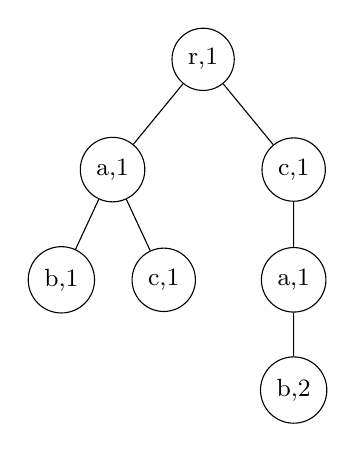
\begin{tikzpicture}[level distance=1.4cm,
  level 1/.style={sibling distance=2.3cm},
  level 2/.style={sibling distance=1.3cm},
  main node/.style={circle,draw,font=\small}]

\node[main node] {r,1}
	child { node[main node] {a,1}
		child { node[main node] {b,1} }
		child { node[main node] {c,1} }
	}
	child { node[main node] {c,1} 
		child { node[main node] {a,1}
			child { node[main node] {b,2} }
		}
	};


\end{tikzpicture}
}
\end{center}

\caption{The CCT of figure~\ref{callex1}. Nodes are labeled in this way: function name, counter.}
\label{cct1}

\end{figure}
\begin{lstlisting}[language=java, caption=An algorithm for building a CCT, morekeywords={function,then,endif},frame=leftline,framesep=10pt]

node treeRoot=null,currentNode=null

function func_call_event_handler(funcType func):

	if (currentNode == null) then 	
		currentNode = new node(func,1) 
		treeRoot=currentNode
		return
	endif

	node temp = currentNode.findNodeByFuncInChildren(func)

	if (temp == null) then
		temp = new node(func,1)
		currentNode.addChildren(temp)
	else
		temp.incrementCounter()
	endif

	currentNode=temp

function func_ret_event_handler():
	currentNode=currentNode.getParent()

\end{lstlisting}

The above code should be self-explaining.
The algorithm for extracting $k$-contexts from a CCT is a little more articulated 
and its pseudo-code will not be shown here but the idea is: given a CCT and a node $n$ of it, it is possible to get the $k$-context of $n$ taking the first (or at most) $k$ nodes from the path which joins $n$ with the root node; doing this for every node and summing counters of all distinct paths is enough for collecting all $k$-contexts of a CCT.

\section{The $k$-Calling Context Forest}

As told in \emph{k-Calling Context Profiling}~\cite{kccf}, building (and handling) a CCT for a relatively long running program is impractical and often useless.
A much better data structure for handling $k$-contexts is \emph{$k$-CCF}: 
the idea on which it is based is to have a \emph{forest} formed by 
a tree (of at most $k$ levels) \emph{for each} function. 

\begin{figure}[h]

\begin{center}
\scalebox{0.8}{
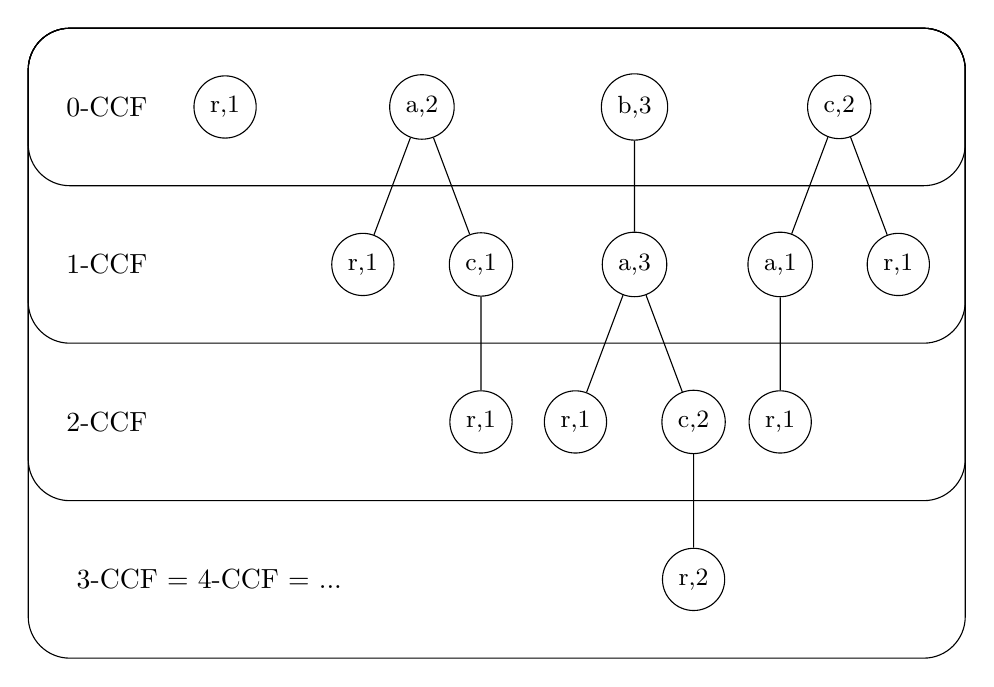
\begin{tikzpicture}[level distance=2.0cm,
  level 1/.style={sibling distance=1.5cm},
  level 2/.style={sibling distance=1.5cm},
  main node/.style={circle,draw,font=\small}]
  

  \node[main node] at (0, 0) {r,1};

  \node[main node] at (2.5, 0) {a,2} 
    child {
	   node[main node] {r,1}
    }
	child {
		node[main node] {c,1}
		child { node[main node]{r,1} }
	};


  \node[main node] at (5.2, 0) {b,3}
  child {
		node[main node] {a,3}
		child { 
			node[main node] {r,1}
		}
		child {
			node[main node] {c,2}
			child { node[main node] {r,2} }
		}
  };

  \node[main node] at (7.8, 0) {c,2}
  child {
		node[main node] {a,1}
		child { node[main node]{r,1} }
  }
  child { node[main node] {r,1} };

  \draw [rounded corners=15pt] (-2.5,-1) rectangle (9.4,1);
  \draw [rounded corners=15pt] (-2.5,-3) rectangle (9.4,1);
  \draw [rounded corners=15pt] (-2.5,-5) rectangle (9.4,1);
  \draw [rounded corners=15pt] (-2.5,-7) rectangle (9.4,1);

  \node at (-1.5,0) {$0$-CCF};
  \node at (-1.5,-2) {$1$-CCF};
  \node at (-1.5,-4) {$2$-CCF};
  \node at (-0.2,-6) {$3$-CCF = $4$-CCF = ...};

\end{tikzpicture}
}
\end{center}

\caption{$k$-CCF relative to CCT in fig.~\ref{cct1} for various values of $k$.}
\label{kccf1}

\end{figure}

The interpretation of fig.~\ref{kccf1} is simple: for $k=0$ there is no context
information and only one node per function is present; its counter shows the number of times that function has been called during the program execution. For $k=1$, every function has as children its callers, for example, $a()$ has been called $2$ times: 1 by $r()$ and 1 by $c()$. This way of proceeding can be extended for greater values of $k$ with the remark that 
there is always a maximum $k$-value which produces a full context-sensitive information 
(in this example, that value of $k$ is $3$): greater values of $k$ have no effect on the output. Apart of these considerations, $k$-CCF have not been formally defined yet because its definition uses an operation called \emph{tree join}.

\subsection{The join operation}

\textbf{Definition 4} \emph{Tree join}~\cite{kccf}. 
The join of two labeled trees $T_1$ and $T_2$, denoted as 
\texttt{\textbf{join(}}$T_1$\texttt{\textbf{,}}$T_2$\texttt{\textbf{)}}, 
is the minimal labeled forest $F$ such that $F$ contains a root-label path $\pi$ if and 
only if $T_1$ or $T_2$ contain $\pi$.

Note: if $T_1$ and $T_2$ have different root labels, 
formally if $l(r_1)\ne l(r_2)$, then $F$ will be simply a forest with two trees: $T_1$ and $T_2$. In order to deals with weighted trees, the join operation just defined have to be extended in this way: \\
\textbf{Definition 4*} \emph{Weighted tree join}~\cite{kccf}.
Let: 

\renewcommand{\labelitemi}{$-$}

\begin{itemize*}
\item $T_1$ and $T_2$ be two trees
\item $V_1$ and $V_2$ be all nodes of $T_1$ and $T_2$
\item $c(v)$ be a counter associated with each node $v$ in $V_1$ and $V_2$
\item $F$ be the weighted tree join of $T_1$ and $T_2$
\item $z$ be a node of $F$
\item $\pi_z$ be the unique root-path that leads to $z$ in $F$
\end{itemize*}
\renewcommand{\labelitemi}{$\bullet$}
$c(z)$ is defined as sum of all counters $c(v)$ of nodes $v$ in $V_1 \cup V_2$ such
that the root-path $\pi_z$ that leads to $v$ in $T_1$ or $T_2$ has the same sequence of 
labels as $\pi_z$.

\begin{figure}[h]

\begin{center}
\scalebox{0.9}{

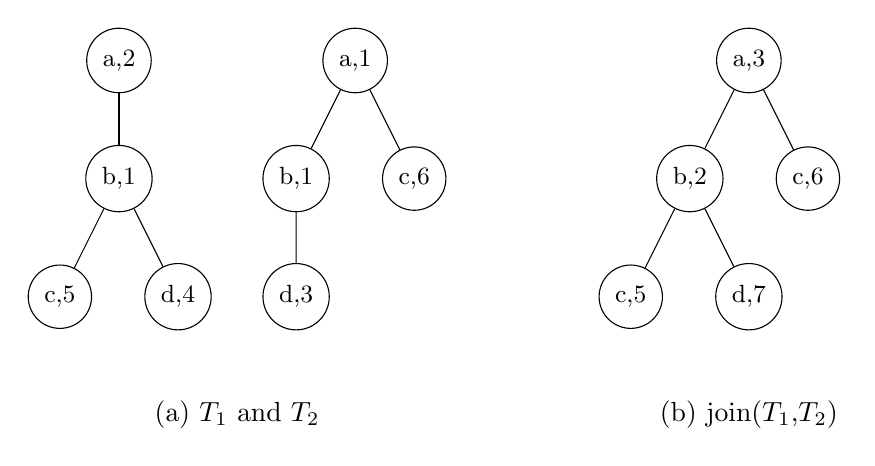
\begin{tikzpicture}[level distance=1.5cm,
  level 1/.style={sibling distance=1.5cm},
  level 2/.style={sibling distance=1.5cm},
  main node/.style={circle,draw,font=\small}]
  
  \node[main node] at (0,0) {a,2}
  child { 
		node[main node] {b,1}
		child {node[main node] {c,5}}
		child {node[main node] {d,4}}
  };

  \node[main node] at (3, 0) {a,1}
  child {
		node[main node] {b,1}
		child {node[main node] {d,3}}
  }
  child {
		node[main node] {c,6}
  };

  \node[main node] at (8, 0) {a,3}
  child {
		node[main node] {b,2}
		child {node[main node] {c,5}}
		child {node[main node] {d,7}}
  }
  child {node[main node] {c,6}};

  \node at (1.5, -4.5) { (a) $T_1$ and $T_2$ };
  \node at (8, -4.5) { (b) join($T_1$,$T_2$) };

\end{tikzpicture}
}
\end{center}

\caption{An example of the tree join operation}
\label{join1}
\end{figure}

Figure~\ref{join1} shows an example that should clarify the above definition:
$T_1$ and $T_2$ trees have a common root-node label, $a$, so they can be merged and 
both counters of $a$ can be summed; also, in both trees is present a path $\langle a,b\rangle$ so the counter of node $a\rightarrow b$ in the resulting tree 
is the sum of the counters of that path in trees $T_1$ and $T_2$; 
the same logic can be used for node $a\rightarrow b\rightarrow d$. 
Instead, paths $\langle a, b, c\rangle$ and $\langle a, c\rangle$ are not common 
in both trees so they exist in the merged tree, but no counters are summed.

The join operation can be extended for working with more than two trees.
let ($T_1$, ..., $T_h$), with $h > 2$, be a set of trees, then:
if all them have distinct root labels, the output forest $F$ will be the same
set of trees, otherwise, if for example $T_1$ and $T_2$ have the same root label,
the following expression could be written:
\begin{center}
\texttt{join($T_1$, \dots, $T_h$) $=$ join(join($T_1$,$T_2$),$T_3$, \ldots, $T_h$)}
\end{center}

\subsection{The formal definition of $k$-CCF}

At this point, $k$-CCF can be formally defined using its original definition.\\

\textbf{Definition 5} \emph{k-Calling Context Forest}~\cite{kccf}. The $k$-calling context
forest of the execution of a program is a labeled forest defined as 
\texttt{join}($\pi_1^R$, \ldots, $\pi_s^R$), where ($\pi_1$, \ldots, $\pi_s$) is the set of
all distinct paths of length a most k+1 activated by the execution\footnote{The notation $\pi^R$ is used for \emph{reverse}-paths}.

\subsection{How to build a $k$-CCF}

Until now, only an basilar explanation of \emph{what} is $k$-CCF was provided; 
now, a first simply way of building it is going to be shown.\\
As previously stated, the CCT of a program execution contains all $k$-contexts for
all possible values of $k$ so, should exist a way to build a $k$-CCF from a CCT: in fact, this is true and can be obtained using a particular operation called $k$-inverse forest, formally defined below.\\

\textbf{Definition 6} \emph{$k$-inverse forest}~\cite{kccf}. Let $F$ be a labeled forest with $n$ nodes
$v_1$, \ldots ,$v_n$. For all $i \in [1,n]$, let $\pi_i$ be the maximal suffix of length at most $k+1$ of the unique root path that leads to $v_i$ in $F$. The $k$-inverse forest of $F$, denoted as $inv_k(F)$, is the labeled forest obtained as \texttt{join}($\pi_1^R$, \ldots ,$\pi_n^R$).\\[20pt]
Now, a $k$-CCF can be build from a CCT using the following property:
\begin{center}
$k$-CCF $=$ $inv_k$(CCT)
\end{center}

The problem of this approach, as already stated before, is that building a CCT 
is \emph{not} space-efficient: it contains all $k$-contexts for every value of $k$ when,
$k$-CCF needs only information about a specific value of $k$. 
Here comes another novel data structure called \emph{$k$-Slab Forest}: 
instead of building a CCT from a program's execution trace, a $k$-SF can be build saving a great amount of space.\\

\section{The $k$-Slab Forest}

A good way to introduce the $k$-SF is by showing its original definition:\\

\textbf{Definition 7} \emph{$k$-Slab Forest}~\cite{kccf}. 
Let $v_1,\ldots,v_t$ be the t nodes at levels multiple of $k$ in the CCT 
(including the root, which has level 0). For any $k > 0$ and each $i \in [1,t]$, let 
$T_{v_i}$ be the maximal subtree of the CCT of depth at most $2k-1$ rooted at $v_i$.
The $k$-slab forest, denoted as $k$-SF, is the labeled forest defined by 
\texttt{join}($T_{v_1}$,\ldots,$T_{v_t}$).\\

The above definition expresses $k$-SF in terms of how it can be build from a CCT.
In a simpler terminology, considering only nodes of a CCT at levels multiple of $k$ (like 0, k, 2k, ...) and their subtrees (of depth at most $2k-1$), it is possible to obtain a $k$-SF by joining all them.

\subsection{Building a $k$-SF from a CCT}

\begin{figure}[h]

\begin{center}
\scalebox{1.0}{

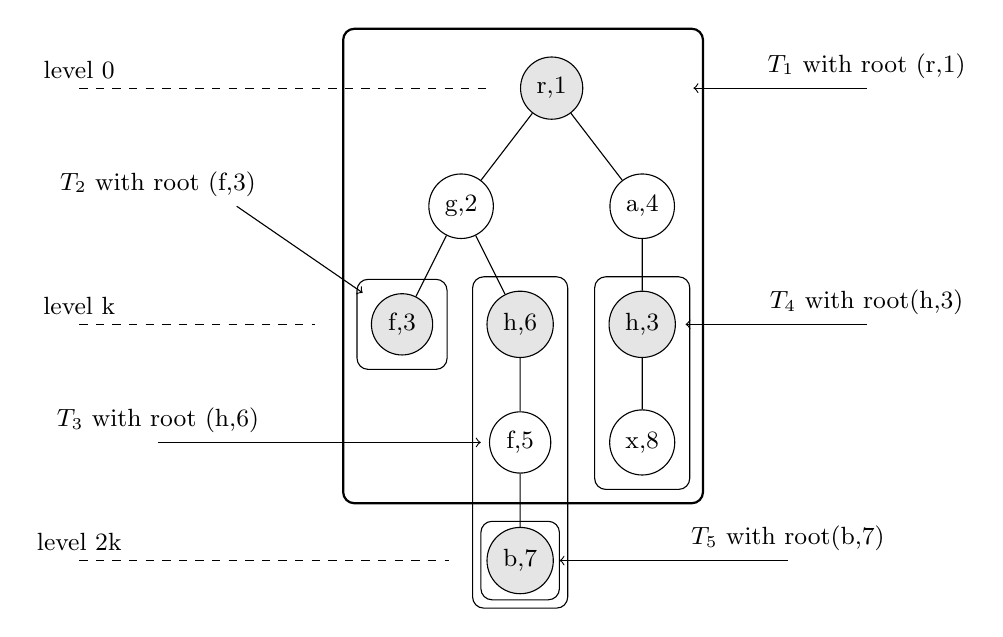
\begin{tikzpicture}[level distance=1.5cm,
  level 1/.style={sibling distance=2.3cm},
  level 2/.style={sibling distance=1.5cm},
  every node/.style={circle,draw,font=\small},
  knode/.style={fill=black!10},
  tnode/.style={above, draw=none, rectangle},
  every fit/.style = {draw, black, inner sep = 5pt, rectangle, rounded corners, thin}]
  
  \node (n0) [knode] at (0,0) {r,1}
  child { 
		node {g,2}
		child {node (n4) [knode] {f,3}}
		child {node (n1) [knode]  {h,6}
			child { node (n2) {f,5}
				child { node [knode] (n3) {b,7} }
			}
		}
  }
  child { node {a,4}
		child { node (n5) [knode] {h,3} 
			child { node (n6) {x,8} }
		}
  };

\node[fit=(n1) (n2) (n3)] {};
\node[fit=(n4)] {};
\node[fit=(n5) (n6)] {};
\node[fit=(n3), inner sep=2pt ] {};
\node[fit=(n0) (n2) (n6) (n4), inner sep=10pt, thick] {};

\draw [dashed] (-6,0) -- (-0.8,0) node [tnode, at start] {level 0};
\draw [dashed] (-6,-3) -- (-3,-3) node [tnode, at start]  {level k};
\draw [dashed] (-6,-6) -- (-1.3,-6) node [tnode, at start] {level 2k};

\draw [<-] (1.8,0) -- (4,0) node[tnode] {$T_1$ with root (r,1)};
\draw [->] (-4,-1.5) -- (-2.4,-2.6) node[tnode] at (-5, -1.5) {$T_2$ with root (f,3)};
\draw [->] (-5, -4.5) -- (-0.9, -4.5) node[tnode, at start] {$T_3$ with root (h,6)};
\draw [<-] (1.7, -3) -- (4, -3) node[tnode] {$T_4$ with root(h,3)};
\draw [<-] (0.1, -6) -- (3, -6) node[tnode] {$T_5$ with root(b,7)};
\end{tikzpicture}
}
\end{center}

\caption{A CCT with its $k$-level subtrees in evidence}
\label{cct2}
\end{figure}

Figure~\ref{cct2} illustrates a CCT and all its 5 subtrees at levels multiple of $k=2$.
Now, the $2$-SF of this CCT can be obtained by computing \texttt{join}($T_1$,\dots,$T_5$).
As fig.~\ref{ksf1} shows, the result is a forest with 4 trees: the first one is exactly $T_1$ because no other subtree has $r$ as root-label; the second one is that obtained by \texttt{join}($T_3$,$T_4$) and then last two ones are the one-node trees $T_2$ and $T_5$ which have not been joined because of their unique root-labels.

\begin{figure}[h]

\begin{center}
\scalebox{0.8}{

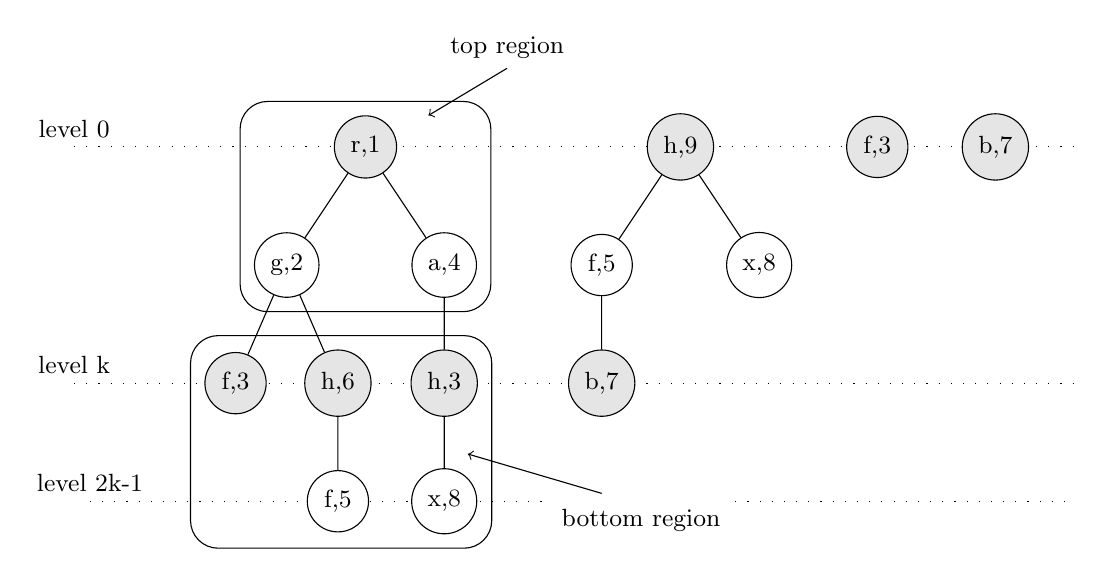
\begin{tikzpicture}[level distance=1.5cm,
  level 1/.style={sibling distance=2.0cm},
  level 2/.style={sibling distance=1.3cm},
  every node/.style={circle,draw,font=\small, radius=1, fill=white},
  knode/.style={fill=black!10},
  tnode/.style={above, draw=none, rectangle},
  every fit/.style = {draw, black, inner sep = 5pt, 
						rectangle, rounded corners=10pt, thin, fill=none}]
 
%\pgfdeclarelayer{back}
%\pgfsetlayers{back,main}

%\begin{pgfonlayer}{back}

\begin{scope}[on background layer]

\draw [loosely dotted] (-3.7,0) -- (9,0) node [tnode, at start] {level 0};
\draw [loosely dotted] (-3.7,-3) -- (9,-3) node [tnode, at start]  {level k};
\draw [loosely dotted] (-3.5,-4.5) -- (9,-4.5) node [tnode, at start] {level 2k-1};

\end{scope}
%\end{pgfonlayer}
 
  \node (n0) [knode] at (0,0) {r,1}
  child { 
		node (g2) {g,2}
		child {node (n4) [knode] {f,3}}
		child {node (n1) [knode]  {h,6}
			child { node (n2) {f,5} }
		}
  }
  child { node (a4) {a,4}
		child { node (n5) [knode] {h,3} 
			child { node (n6) {x,8} }
		}
  };

  \node [knode] at (4,0) {h,9}
  child { node {f,5} child { node [knode] {b,7} }}
  child { node {x,8} };

  \node [knode] at (6.5, 0) {f,3};
  \node [knode] at (8, 0) {b,7};

\node [fit = (n4) (n1) (n5) (n2) (n6)] {};
\node [fit = (n0) (g2) (a4)] {};

\draw [<-] (0.8,0.4) -- (1.8,1) node[tnode] {top region};
\draw [<-] (1.3,-3.9) -- (3, -4.4) node[tnode] at (3.5,-5) {bottom region};

\end{tikzpicture}
}
\end{center}

\caption{The $2$-SF relative to fig.~\ref{cct2}}
\label{ksf1}
\end{figure}

Now, $k$-SF has been defined and a way for building it from a CCT is shown but,
should be clear at this point that this method for building the $k$-SF is useless because
the $k$-CCF itself can be build directly from the CCT: the goal is to build $k$-SF \emph{without} a CCT and then to build the $k$-CCF from the $k$-SF. 

\subsection{Building a $k$-SF without a CCT}

The algorithm for building \emph{online} the $k$-SF is similar to the one purposed for building CCT but, instead of having 
one single \verb|currentNode| pointer (and, of course, only one tree), there two are pointers (\verb|top| and \verb|bottom|) that work at the same time on two different regions: \emph{top} region and \emph{bottom} region as shown in fig.~\ref{ksf1}.
Besides the two pointers and the $k$-SF, the algorithm uses:

\begin{itemize}
\item \verb|R|, a hashset which contains root pointers of all $k$-SF trees indexed by node label in a way that, given a label, it is possible to access its node-pointer in $O(1)$.

\item A shadow stack \verb|S| used for storing $\langle$top,bottom$\rangle$ pairs relative to each routine activation. 
\end{itemize}

At the algorithm start, \verb|S| contains a special pair of \verb|null| pointers; 
at the first procedure call, the \verb|if| condition on line 15 is verified:
the algorithm creates the root-node, makes \verb|top| pointing on it and adds also that pointer in \verb|R|. In the following procedure calls, the \verb|top| pointer is updated exactly as the \verb|currentNode| pointer in the CCT building algorithm (lines 36-46) except when \verb|S.size()-1| is a multiple of $k$: in that case (lines 16-34), \verb|bottom| is moved to \verb|top| and \verb|top| is moved to a (possibly) new tree of the forest; when the ``new'' tree already exists (this information is provided by \verb|R|), \verb|top| is simply moved to its root (line 25). After the first time \verb|top| is moved, the pointer \verb|bottom| is not more \verb|null| and is updated as the \verb|currentNode| pointer in CCT (lines 54-66). 

\begin{lstlisting}[language=java, caption=An algorithm for building a $k$-SF,
			morekeywords={function,then,endif},
			frame=leftline,framesep=10pt,numbers=left, numbersep=15pt]

stack S
hashset R
forest kSF
node top=null,bottom=null

function init:
	S.push( (null,null) )

function func_call_event_handler(funcType func):

	(top,bottom) = S.top()
	
	/* update top region */
	if ( ( (S.size()-1) mod k ) == 0 ) then

		/* bottom is moved to top and top to a "new" tree */

		bottom=top
		node temp = R.find( func )

		if (temp == null) then

			/* a tree with label "func" does not exist */
			node n2 = new node( func, 0 )
			kSF.addTree(n2)
			R.add(n2)
			top=n2
		else

			/* a tree with label "func" already exists */
			top = temp
		endif

	else

		/* regular top pointer update */

		node temp = top.findNodeByFuncInChildren( func )

		if (temp == null) then
			temp = new node( func, 0 )
			top.addChildren( temp )
		endif

		top = temp

	endif

	top.incrementCounter()

	/* update bottom region */
	if (bottom != null) then
		
		/* regular bottom pointer update */

		node temp = bottom.findNodeByFuncInChildren( func )
		
		if (temp == null) then
			temp = new node( func, 0 )
			bottom.addChildren( temp )
		endif

		bottom = temp
		bottom.incrementCounter()

	endif

	/* top and bottom pointers are saved on the stack */
	S.push( (top, bottom) )

function func_ret_event_handler():

	/* 
		the last procedure returned, so its record 
		on the shadow stack is removed 
	*/
	
	S.pop()

\end{lstlisting}


\subsection{Building a $k$-CCF from a $k$-SF}

A $k$-CCF can be build from a $k$-SF using the following fundamental property of $k$-SF:
\begin{center}
$k$-CCF $=$ $inv_k$($k$-SF)
\end{center}
This means that a $k$-CCF can be obtained from a $k$-SF using the \emph{same} operation
used on a CCT, as if $k$-SF were a generalization of CCT: this is true and in fact, for $k\rightarrow \infty$, $k$-SF = CCT~\cite{kccf}.
There is only a problem in using the above property: the $k$-CCF build in that way has \emph{wrong} counters. The cause of that is the intrinsic data duplication in $k$-SF when a new tree is added by moving the \verb|top| pointer: \verb|top| and \verb|bottom| pointers build the same subtree in different places and both increment their counters. Of course, there is a solution: before applying $inv_k$ to $k$-SF, all counters of top regions of $k$-SF, except for the first tree, must be cleared to zero. The figure below shows that operation applied to the $k$-SF on fig.~\ref{ksf1}.


\begin{figure}[h]

\begin{center}
\scalebox{0.8}{

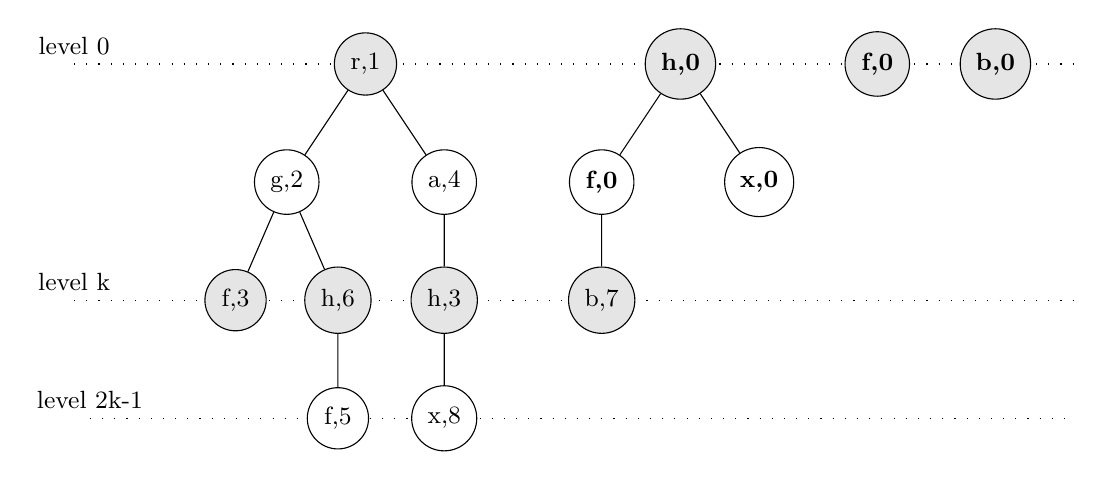
\begin{tikzpicture}[level distance=1.5cm,
  level 1/.style={sibling distance=2.0cm},
  level 2/.style={sibling distance=1.3cm},
  every node/.style={circle,draw,font=\small, radius=1, fill=white},
  knode/.style={fill=black!10},
  tnode/.style={above, draw=none, rectangle},
  every fit/.style = {draw, black, inner sep = 5pt, 
						rectangle, rounded corners=10pt, thin, fill=none}]
 
%\pgfdeclarelayer{back}
%\pgfsetlayers{back,main}

%\begin{pgfonlayer}{back}

\begin{scope}[on background layer]

\draw [loosely dotted] (-3.7,0) -- (9,0) node [tnode, at start] {level 0};
\draw [loosely dotted] (-3.7,-3) -- (9,-3) node [tnode, at start]  {level k};
\draw [loosely dotted] (-3.5,-4.5) -- (9,-4.5) node [tnode, at start] {level 2k-1};

\end{scope}
%\end{pgfonlayer}
 
  \node (n0) [knode] at (0,0) {r,1}
  child { 
		node (g2) {g,2}
		child {node (n4) [knode] {f,3}}
		child {node (n1) [knode]  {h,6}
			child { node (n2) {f,5} }
		}
  }
  child { node (a4) {a,4}
		child { node (n5) [knode] {h,3} 
			child { node (n6) {x,8} }
		}
  };

  \node [knode] at (4,0) {\textbf{h,0}}
  child { node {\textbf{f,0}} child { node [knode] {b,7} }}
  child { node {\textbf{x,0}} };

  \node [knode] at (6.5, 0) {\textbf{f,0}};
  \node [knode] at (8, 0) {\textbf{b,0}};

%\node [fit = (n4) (n1) (n5) (n2) (n6)] {};
%\node [fit = (n0) (g2) (a4)] {};

%\draw [<-] (0.8,0.4) -- (1.8,1) node[tnode] {top region};
%\draw [<-] (1.3,-3.9) -- (3, -4.4) node[tnode] at (3.5,-5) {bottom region};

\end{tikzpicture}
}
\end{center}

\caption{The $k$-SF of fig.~\ref{ksf1} with cleared counters in top regions}
\label{ksf2}
\end{figure}

\section{Final remarks}

In this chapter, $k$-CCF and $k$-SF data structures have been only \emph{basically} explained: many of their properties and theorems about them have been voluntarily omitted; 
also, no proofs neither any kind of space\slash time analysis have been shown.
This is because the goal of this chapter was only to explain what \emph{practically} $k$-CCF and $k$-SF are and how they can be \emph{technically} used in profilers such as IHPP. 

The author invites readers who really want to understand these data structures and their theoretical implications to read the original work \emph{k-Calling Context Profiling}~\cite{kccf}.


\chapter{An Intraprocedural Hot Path Profiler}

IHPP is a profiler written in C++. Technically it is not a program but
 a \emph{plug-in}\footnote{In the pin-specific slang,
plug-ins like IHPP are called \emph{pintools}.} for the tool 
Intel \textbf{Pin}\footnote{Official page: \url{http://www.pintool.org}}.
This last one, is a dynamic binary instrumentation framework for the IA-32 and x86-64 instruction-set architectures that allows the creation of dynamic program analysis tools. 
Pintools have, through pin, the full control of a target program: 
when this one is loaded in memory, all its routines and instructions are visible
to the pintool: it can modify or simply \emph{instrument} them. 
Instrumenting a routine means adding a \verb|call| instruction to a pintool analysis 
routine at its beginning; also, it is possible to instrument \verb|ret| instructions 
in order to catch \verb|return| statements of the target program: 
in this way a tool can build, for example, the program's CCT.
In this chapter, basics of IHPP such as its working modes and how can be used will be explained with a few technical considerations.

\section{An overview of IHPP}

IHPP has three main working modes: \emph{function}-mode, \emph{intra}-procedural mode and \emph{inter}-procedural mode. 

\begin{paragraph}{The function mode}
In this mode, IHPP builds a $k$-SF and a $k$-CCF for every thread of a program,
with an option (called \verb|joinThreads|) to join all $k$-SFs and produce a cumulative $k$-SF-$k$-CCF couple relative to the program execution.
This working mode is almost a direct application of the concepts explained in chapter 3. 
\end{paragraph}

\begin{paragraph}{The intra-procedural mode}
This other mode instead, deals with \emph{basic blocks} (from now called BBLs) inside procedures: the concept of \emph{calling a function} is transformed in the \emph{entering in a BBL}, while the concept of \emph{returning from a function call} totally disappears in this working mode; BBLs have no stack information and so, it is impossible to ``return'' to a previously activated BBL instance: it is only possible to activate this BBL again though a loop or a \verb|goto| statement.
IHPP instruments all BBLs inside chosen functions of a program and produces in output a couple $k$-SF-$k$-CCF for each function executed within each thread. The \verb|joinThreads| option is available also in this mode: it joins all $k$-SFs relative to a function generated by all threads in which that function has been called, for each function.
Another important feature in \emph{intra}-procedural mode is the \verb|rollLoops| option: it substantially produces $\infty$-SFs which do not grow due to loops inside functions because they are recognized and as result only counters are incremented. 
\end{paragraph}

\begin{paragraph}{The inter-procedural mode}
Despite of its name (\emph{intra}procedural profiler), IHPP has also a particular and unique working mode that deals with BBLs but in which the concept of \emph{procedure} is totally removed. In this working mode, a program is composed only by BBLs: there are no functions, so no calls and no returns. IHPP builds a couple of $k$-SF-$k$-CCF for each thread as other modes, but it is like the program has only one big procedure. This mode can be useful, for example, when one wants to analyze an algorithm implemented with two or more functions without considering the caller-callee relations but focusing the attention on execution flow of the hole algorithm. In the case when only one function is instrumented, there is no difference between \emph{inter-} and \emph{intra-} procedural modes.
\end{paragraph}

\subsection{Technical considerations}

Like Pin itself, IHPP works both on Microsoft \textbf{Windows} and \textbf{Linux}-based systems but, output data sometimes is different and the reason is the compiler: 
under Linux systems the compiler \verb|gcc| is supported instead, under Windows only the compiler \verb|cl| included in the software \textbf{Visual Studio} is supported. 
This means that both the IHPP and the target program have to be compiled with the same compiler under a specific platform. Under Windows systems, target programs built with \verb|gcc| portings or other compilers are not supported due to problems with debug information: 
practically, IHPP fetches the debug information of a program through Pin which accepts only \verb|pdb| debug info format under Windows and only \verb|dwarf| format under Linux-based systems; but, the problematic difference between the two compilers is another: 
they compile C/C++ code in a different way and often they do not respect the \emph{standard calling conventions}, specially in auxiliary routines inserted into the target program. 
Because of this, a huge amount of work has been done in IHPP to overcome these problems, 
specially under Windows systems.

\section{The \emph{function} mode}

As said before, \emph{function} mode (internally called \verb|funcMode|) 
is a way of profiling very similar to the one theoretically explained in chapter 3.
A concrete example will be helpful to show this.

\begin{lstlisting}[language=C, 
	caption={prog1.c, a simple multi-threaded program}, label=prog1, frame=leftline]

#include <stdio.h>
#include <stdlib.h>
#include <pthread.h>

void a(); void b(); void c();
void d(); void e();

void a() { b(); c(); }
void b() { }
void c() { }
void d() { c(); c(); }
void e() { d(); c(); a(); }

void *thread2_func(void *arg) { a(); return 0; }

int main(int argc, char ** argv) {

	pthread_t th;

	a(); e(); e();

	pthread_create(&th, NULL, thread2_func, NULL);
	pthread_join(th, NULL);
	return 0;
}

\end{lstlisting}

\flushleft
Compiling the example program in \cref{prog1} under a Linux system with:
\begin{center}
\verb|gcc -g prog1.c -o prog1 -lpthread|
\end{center}
and starting IHPP with\footnote{Due to permission problems under Linux pin have to be run with the \texttt{-injection child} option before the \texttt{-t} option. See its official user manual for an explanation.}:
\begin{center}
\begin{verbatim}
pin -t ihpp.so -ksf -kinf -funcMode -outfile out1.txt -- ./prog1
\end{verbatim}
\end{center}

will produce as output a file called \verb|out1.txt|\footnote{Some lines have been removed for compactness.}:\\[20pt]

\begin{lstlisting}[label=out1, caption=File out1.txt]

K value: INFINITE
====================================================================
Thread ID: 4294967296
====================================================================
--------------------------------------------------------------------
DUMP of K-SF
--------------------------------------------------------------------

| _start(),1
   | __libc_csu_init(),1
      | __i686.get_pc_thunk.bx(),1
      | _init(),1
         | frame_dummy(),1
         | __do_global_ctors_aux(),1
   | main(),1
      | a(),1
         | b(),1
         | c(),1
      | e(),2
         | d(),2
            | c(),4
         | c(),2
         | a(),2
            | b(),2
            | c(),2
   | _fini(),1
      | __do_global_dtors_aux(),1
====================================================================
Thread ID: 8589934593
====================================================================
--------------------------------------------------------------------
DUMP of K-SF
--------------------------------------------------------------------

| thread2_func(),1
   | a(),1
      | b(),1
      | c(),1
\end{lstlisting}


A few considerations. 
\renewcommand{\labelitemi}{$-$}

\begin{itemize*}
\item The program is multi-threaded and IHPP correctly shows this 
producing two different $k$-SFs. 
\item Only $k$-SFs are present in output because IHPP has been called without the \verb|-kccf| option.
\item $k$-SFs shown are in fact CCTs because \verb|-kinf| option is used.
\item The are some compiler routines that almost always will not be an object of interest for an user of IHPP. Note: programs compiled with \verb|cl| under Windows have \emph{hundreds} of compiler\slash library routines even if, of course, the program \emph{is not} compiled with \emph{static} linking of standard libraries. 
\end{itemize*}

\renewcommand{\labelitemi}{$\bullet$}

Instead, executing IHPP on the same program specifying this time the list 
of functions to instrument with \verb|-funcs a,b,c,d,e| the output written to \verb|out2.txt| will be:

\begin{lstlisting}[label=out2, caption=File out2.txt]
K value: INFINITE
====================================================================
Thread ID: 4294967296
====================================================================
--------------------------------------------------------------------
DUMP of K-SF
--------------------------------------------------------------------

| __root__(),1
   | a(),1
      | b(),1
      | c(),1
   | e(),2
      | d(),2
         | c(),4
      | c(),2
      | a(),2
         | b(),2
         | c(),2
====================================================================
Thread ID: 8589934593
====================================================================
--------------------------------------------------------------------
DUMP of K-SF
--------------------------------------------------------------------

| __root__(),1
   | a(),1
      | b(),1
      | c(),1
\end{lstlisting}

It is clear that reading this output is easier than reading output in \cref{out1} but,
another thing comes out: there is \verb|__root__|, a ``new'' function not shown before.
It is not a really function but only a \emph{fake} symbol that IHPP automatically adds
as root of the first tree for each thread. The reason is simple: when an user specifies 
a list of functions, there is absolutely no guarantee that among these one is a relative root function.
One criticism towards this solution can be to say that $k$-SF is a \emph{forest}, not a tree, so the fake root node can be avoided: the answer is that criticism is wrong because of two reasons:
\begin{enumerate}
\item $\infty$-SF is a CCT \emph{by definition}: without the fake root $\infty$-SF will still be a forest and not a \emph{calling context tree}. 
\item Since $k$-SF will be wrong without a fake root (for all values of $k$ greater than a certain $\bar{k}$), a correct $k$-CCF could not be generated: as explained in chapter 3, before the $inv_k$ operation, counters of all nodes
in top regions must be cleared with the exception of the first three, which has as root node, the root of the CCT relative to the program execution trace. In the example above,
neither \verb|a()| nor \verb|e()| is eligible as CCT's root.
\end{enumerate}

\subsection{The \emph{joinThreads} option}

When invoking IHPP with the \verb|-joinThreads| option, after the target program ended
IHPP will join all $k$-SFs together before (eventually) building the $k$-CCF.
The output of IHPP after profiling the program in \cref{prog1} will be:

\begin{lstlisting}[label=out3, caption=File out3.txt]
--------------------------------------------------------------------
DUMP of K-SF
--------------------------------------------------------------------

| __root__(),2
   | a(),2
      | b(),2
      | c(),2
   | e(),2
      | d(),2
         | c(),4
      | c(),2
      | a(),2
         | b(),2
         | c(),2
\end{lstlisting}

\section{The \emph{intra}-procedural mode}

adh ak dj ak jhd a k h a kd h ak d  hk q hd k aj h d  i q h  i k h  ka h dk a h dj s k aj ka j h d  k aj h d akj h da 
adh akdjakjhda khakdhakd hkqhdkajhd iqh ikh kahdkahdjskaj kajhd kajhdakjhda
adh akdjakjhda khakdhakd hkqhdkajhd iqh ikh kahdkahdjskaj kajhd kajhdakjhda
adh akdjakjhda khakdhakd hkqhdkajhd iqh ikh kahdkahdjskaj kajhd kajhdakjhda
adh akdjakjhda khakdhakd hkqhdkajhd iqh ikh kahdkahdjskaj kajhd kajhdakjhda
adh akdjakjhda khakdhakd hkqhdkajhd iqh ikh kahdkahdjskaj kajhd kajhdakjhda
adh akdjakjhda khakdhakd hkqhdkajhd iqh ikh kahdkahdjskaj kajhd kajhdakjhda


\section{The \emph{inter}-procedural mode}

adh akdjakjhda khakdhakd hkqhdkajhd iqh ikh kahdkahdjskaj kajhd kajhdakjhda
adh akdjakjhda khakdhakd hkqhdkajhd iqh ikh kahdkahdjskaj kajhd kajhdakjhda
adh akdjakjhda khakdhakd hkqhdkajhd iqh ikh kahdkahdjskaj kajhd kajhdakjhda
adh akdjakjhda khakdhakd hkqhdkajhd iqh ikh kahdkahdjskaj kajhd kajhdakjhda
adh akdjakjhda khakdhakd hkqhdkajhd iqh ikh kahdkahdjskaj kajhd kajhdakjhda


\chapter{The implementation}



\chapter{Case studies}


\chapter{Conclusions}

\bibliography{bibliography}{}
\bibliographystyle{plain}

\end{document}